\documentclass{beamer}
\setbeamertemplate{section in toc}[sections numbered]
\usefonttheme[onlymath]{serif}
\beamertemplatenavigationsymbolsempty
\setbeamertemplate{footline}{% 
  \hfill% 
  \usebeamercolor[gray!50]{page number in head/foot}% 
  \usebeamerfont{page number in head/foot}% 
  \insertframenumber\,/\,\inserttotalframenumber%
}
\usepackage{amsmath}
\usepackage{graphicx}
% \usepackage{caption}
% \usepackage[skip=0pt]{subcaption}
% \usepackage[tight,FIGTOPCAP]{subfigure}
\usepackage{lmodern}
\usepackage[round]{natbib}
% \usepackage{braket}
\usepackage{color}
\usepackage{bm}
\usepackage{amssymb}
\usepackage{bbold}
\usepackage{tikz}
\usepackage{empheq}
\usepackage{stackengine}
\usepackage{framed}
\usepackage[percent]{overpic}
\usepackage{adjustbox}
\usepackage{simpler-wick}
\usepackage{physics}
\DeclareMathOperator{\sgn}{sgn}
\tikzset{>=latex}
\newcommand{\blue}[1]{{\color{blue}{#1}}}
\newcommand{\md}{\mathrm{d}}
\newcommand{\ms}{\mathsf}
\newcommand{\bs}{\boldsymbol}
\newcommand{\mc}{\mathcal}
\renewcommand{\(}{\left(}
\renewcommand{\)}{\right)}
\renewcommand{\[}{\left[}
\renewcommand{\]}{\right]}

%Information to be included in the title page:
\title{Modeling Electronic Systems on Quantum Computers}
%\author{Apoorv Tiwar, Ammar Jahin, and Yuxuan Wang}
%\institute{University of Florida}
\date{University of Florida, October}

\begin{document}
\frame{\titlepage} 
\AtBeginSection[]
{
\begin{frame}
    \frametitle{Outline}
    \tableofcontents[currentsection]
\end{frame}
}

\begin{frame}
    \frametitle{Recap of last time}
    \begin{itemize}
        \item Jordan-Wigner transformation to map between the fermioinc degrees of freedom and the qubits degrees of freedom. 
        \begin{center}
            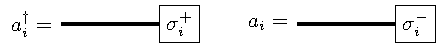
\includegraphics[]{jordan_wigner.pdf}
        \end{center} 
    \end{itemize}
    \begin{columns}
        \begin{column}[]{0.6\textwidth}
            \begin{itemize}
                \item Using JW we have, 
                \begin{align*}
                    a^\dagger_i a_i = \frac{1}{2} (1+\sigma^z_i)
                \end{align*}
                \item In the qubits degrees of freedom the Hamiltonian is a linear combination of polynomial number of Pauli strings. For the Hydrogen molecule case, 
                \begin{align*}
                    \hat{H} = \sum_{i,j,k,l = 0}^ 3 j^{ijkl} \sigma^i_1 \sigma^j_2 \sigma^k_3 \sigma^l_4 
                \end{align*}
            \end{itemize}
        \end{column}
        \begin{column}[]{0.35\textwidth}
            \begin{center}
                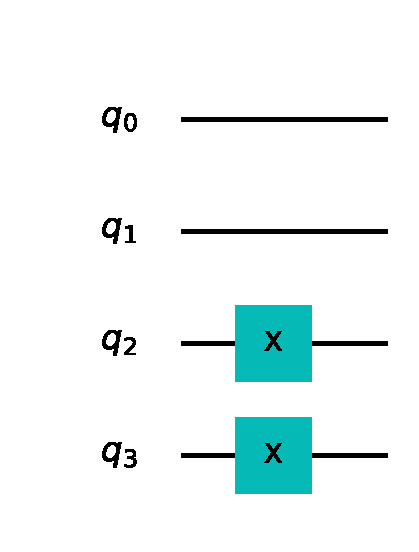
\includegraphics[scale=0.5]{initial_state_r.pdf}
            \end{center} 
        \end{column}
    \end{columns}

\end{frame}

\section{VQE algorithm circuit design for UCCSD}


\begin{frame}
    \frametitle{Unitary coupled-cluser (UCC) expansion}
    The UCC method uses the following ansatz, 
    \begin{columns}
        \begin{column}[]{0.55\textwidth}
            \begin{align*}
                &\ket{\Psi_0} = e^{T(\bm \theta) - T^\dagger (\bm \theta)} \ket{\Phi_0} \\ 
                &T(\bm \theta) = T_1(\bm \theta) + T_2(\bm \theta) + \dots \\ 
                & T_1(\bm \theta) = \sum_{\substack{m\in \text{emp} \\ i \in \text{occ}}} \theta^{mi} a^\dagger_m a_i \\ 
                &T_2(\bm \theta) = \frac{1}{2} \sum_{\substack{m, n\in \text{emp} \\ i, j \in \text{occ}}} \theta^{mnij} a^\dagger_m a^\dagger_n a_i a_j \\
                &  \quad \vdots
            \end{align*}
        \end{column}
        \begin{column}[b]{0.45\textwidth}
            \begin{align*}
                e^{T(\bm \theta) - T^\dagger (\bm \theta)} = e^{\sum_i \theta_i (\tau_i - \tau^\dagger_i)},
            \end{align*}
            where $\tau_i$ include all kinds of excitations. 
        \end{column}
    \end{columns}
    \begin{itemize}
        \item For this ansatz to be computationally efficient we need to include only a few excitation operators. 
        \item UCCSD include single and double excitations.
        \item Next step would be to design a circuit that implement this unitary operation. 
    \end{itemize}
\end{frame}

\begin{frame}
    \frametitle{Trotterization}
    Different terms of $\tau_i$ don't necessarily commute which make simulating the exponential with quantum circuits not easy. 

    We make use of the following identity,
    \begin{align*}
        e^{\sum_i \theta_i (\tau_i - \tau^\dagger_i)} = \lim_{N \rightarrow \infty}\(\prod_i e^{\frac{\theta_i (\tau_i - \tau_i^\dagger)}{N}}\)^N
    \end{align*}
    \pause
    \begin{itemize}
        \item Taking $N$ to infinity is not possible for computations. Good results can be achieved by taking just a few trotter steps.
    \end{itemize}
    \begin{align*}
        e^{\sum_i \theta_i (\tau_i - \tau^\dagger_i)} = \(\prod_i e^{\frac{\theta_i (\tau_i - \tau_i^\dagger)}{\rho}}\)^\rho
    \end{align*}
    \begin{itemize}
        \item The smaller the $\theta_i$'s are the better the approximation.
        \item It's better to start with a good initial guess. 
    \end{itemize}
    
\end{frame}

\begin{frame}
    \frametitle{Converting to qubits operations}
    \framesubtitle{one-body exponentials}

    One body exponential $e^{\theta (a^\dagger_m a_i - a^\dagger_i a_m )}$. Note: $m>i.$ 
    \begin{align*}
        &a^\dagger_m a_i - a^\dagger_i a_m = -\sigma^{-}_i \(\prod_{s=i+1}^{m-1} \sigma_s^z\) \sigma^{+}_m  + \sigma^{+}_i  \(\prod_{s=i+1}^{m-1} \sigma_s^z\) \sigma^{-}_m \\
        % &\sigma^{+} \sigma^{z} = -(\sigma^{-} \sigma^{z})^\dagger = - \sigma^{+} \\ 
        &a^\dagger_m a_i - a^\dagger_i a_m = \frac{i}{2} \[ \sigma^{y}_i \(\prod_{s=i+1}^{m-1} \sigma_s^z\) \sigma^{x}_m  - \sigma^{x}_i \(\prod_{s=i+1}^{m-1} \sigma_s^z\) \sigma^{y}_m \]
    \end{align*}
    Note that the two terms commute. 
    \pause

    We rotate $\sigma^x$ and $\sigma^y$ to $\sigma^{z}$,
    \begin{align*}
        e^{i\theta \sigma^{y}_i \(\prod_{s=i+1}^{m-1} \sigma_s^z\) \sigma^{x}_m}  = H_m R^x_i(\pi/2)\(e^{i\theta \(\prod_{s=i}^{m-1} \sigma_s^z\) \sigma^{z}_m } \)H^\dagger_m R^{x\dagger}_i(\pi/2), 
    \end{align*}
    using,
    \begin{gather*}
        H \sigma_z H^\dagger  = \sigma_x \\ 
        R^x\(\pi/2\) \sigma_z R^{x\dagger}\(\pi/2\)  = \sigma_y 
    \end{gather*}
\end{frame}

\begin{frame}
    \frametitle{Converting to qubit operations}
    \framesubtitle{one-body exponentials}
    Need to implement $\exp\[i\theta \(\prod_{s=i}^{m-1} \sigma_s^z\) \sigma^{z}_m \]$. 
    \begin{itemize}
        \item $\prod_{s=i}^{m-1} \sigma_s^z$ counts the parity of qubits from $i$ to $m-1$. 
        \item $e^{\pm i \theta\sigma^z_m }$ makes a rotation around the $z$-axis on the $m$-th qubit accordingly. 
    \end{itemize}
    \pause
    Example: $\exp\[i\theta \sigma^{y}_1 (\sigma_2^z \sigma_3^z )\sigma^{x}_4 \]$ for Hydrogen molecule.  
    \begin{center}
        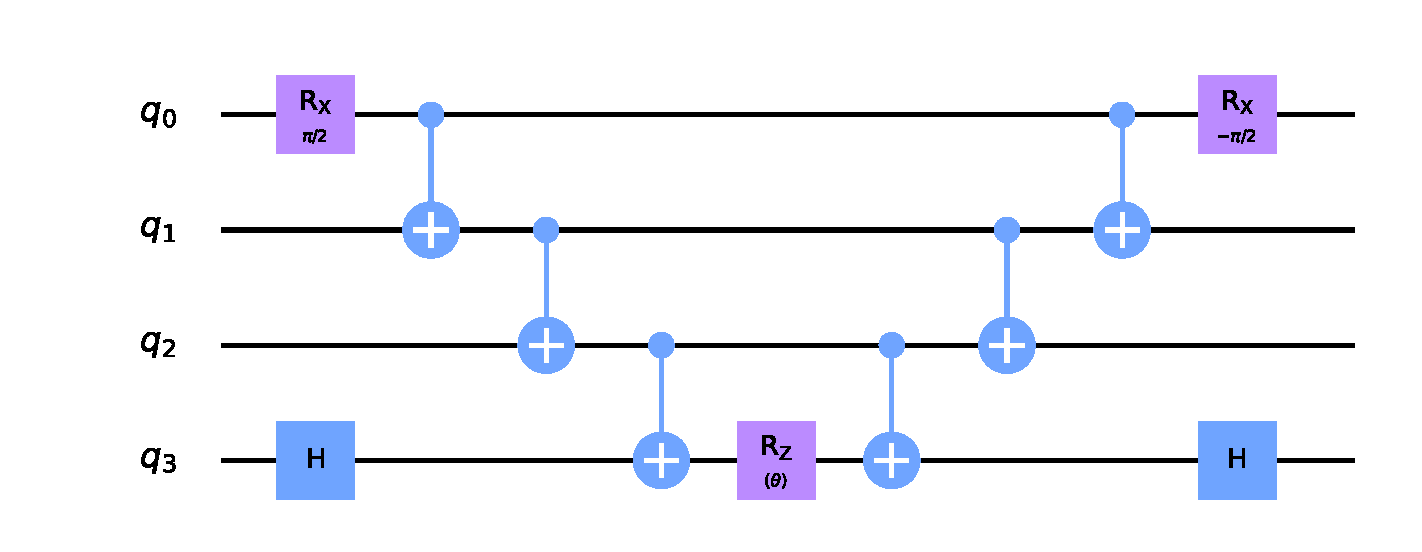
\includegraphics[scale = 0.45, trim = 65 0 0 0 , clip]{a_4a_1_r.pdf} 
    \end{center}
\end{frame}

\begin{frame}
    \frametitle{Converting to qubit operations}
    \framesubtitle{two-body exponentials}

    Two-body exponential $e^{\theta (a^\dagger_m a^\dagger_n a_j a_i - a^\dagger_i a^\dagger_j a_n a_m  )}$, and assume $j>i$, and $m>n$ 

    \begin{align*}
        a^\dagger_m a^\dagger_n a_i a_j - a^\dagger_i a^\dagger_j a_n a_m  = &\sigma^{-}_i \(\prod \sigma^{z}\) \sigma^{-}_j\  \sigma^{+}_n \(\prod \sigma^{z}\) \sigma^{+}_m \\ 
        - & \sigma^{+}_i \(\prod \sigma^{z}\) \sigma^{+}_j\  \sigma^{-}_n \(\prod \sigma^{z}\) \sigma^{-}_m \\ 
        = & \frac{i}{4} \sigma^{x}_i \(\prod \sigma^{z}\) \sigma^{x}_j \  \sigma^{x}_n \(\prod \sigma^{z}\) \sigma^{y}_m \\ 
        + &\text{terms with odd } \sigma^{y} 
    \end{align*}
    This generate $8$ terms, all of which will commute. As before we rotate $\sigma^x$ and $\sigma^y$ to $\sigma^{z}$, 
    \begin{align*}
        H_i H_i H_n R^x_m(\pi/2) e^{\frac{i\theta}{4} \(\(\prod_{i}^{j} \sigma^{z}\)\  \(\prod_{n}^{m-1} \sigma^{z}\)  \sigma^{z}_m \)} H^\dagger_i H^\dagger_i H^\dagger_n R^x_m(-\pi/2)
    \end{align*}
    
\end{frame}

\begin{frame}
    \frametitle{Converting to qubit operations}
    \framesubtitle{two-body exponentials}
    Note we only add parity from $m$ to $n$ and from $j$ to $i+1$ then perform the rotation on the $i$-th qubit.
     
    Example: $\exp{\[ i\theta \sigma^x_1 \sigma^x_2 \sigma^x_3 \sigma^y_4  \ \]}$ for the Hydrogen molecule, 

    \begin{center}
        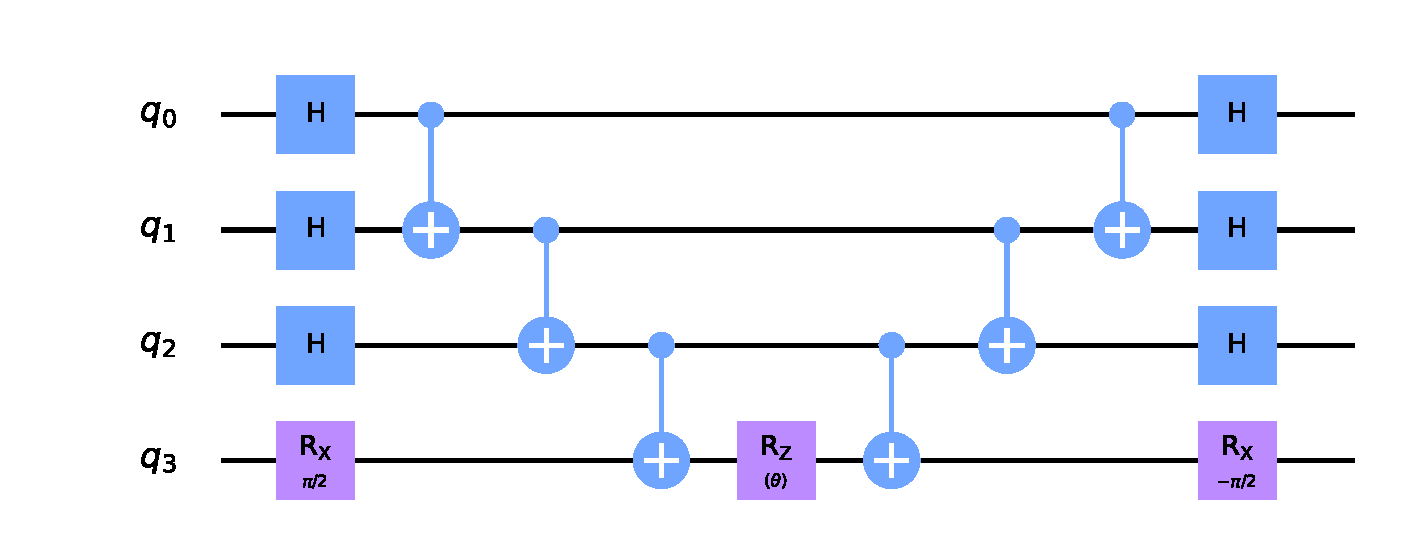
\includegraphics[scale=0.45, trim = 65 0 0 0 , clip]{a1a2a3a4_r.pdf}
    \end{center}
\end{frame}

\begin{frame}
    \frametitle{Measuerment}
    The Hamiltonian expectation value is written as, 
    \begin{align*}
        \ev*{\hat{H}} = \sum_{i,j,k,l = 0}^ 3 j^{ijkl}\ev*{\sigma^i_1 \sigma^j_2 \sigma^k_3 \sigma^l_4} 
    \end{align*}
    The computational basis is the $z$-axis. To measure the expectation value a general string of Pauli operators, we need a post-rotation circuit. 
    \begin{itemize}
        \item Measuring the qubits gives a string of $0$'s and $1$'s, $\{s_i\}$.
        \item $P(\{ s_i \}) = |\braket{\{s_i\}}{\Psi_0}|^2$
        \item To measure the $i$-th qubit with respect to the $x$ or $y$-axes we need to rotate our basis for the $i$-th qubit using $H_i$ or $R_i^{x}(\pi/2)$ respectively. 
        \item Any Pauli string has eigenvalues of either $\pm 1$.
        \item $\ev*{\sigma^i_1 \sigma^j_2 \sigma^k_3 \sigma^l_4} = P(1) - P(-1)$ 
    \end{itemize}
\end{frame}

\begin{frame}
    \frametitle{}
    The end result look something like this: 
    \begin{center}
        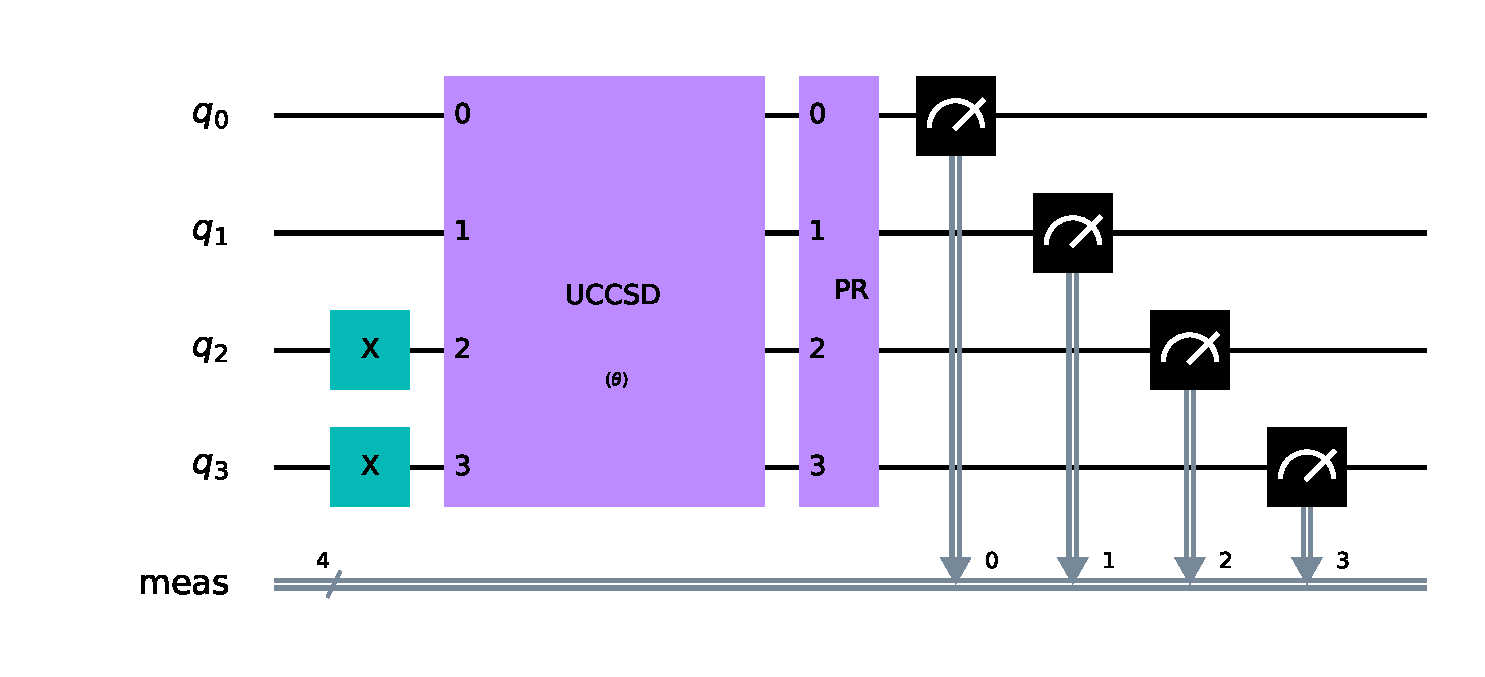
\includegraphics[scale=0.445, trim = 65 0 0 0 , clip]{uccsd_qc.pdf}
    \end{center}
    \begin{columns}
        \begin{column}[]{0.7\textwidth}
            \begin{enumerate}
                \item Initialize the qubits 
                \item Apply the UCCSD gate with parameters $\bm \theta$.
                \item Apply post-rotations.
                \item Measure the qubits.
            \end{enumerate}
        \end{column}
        \begin{column}[]{0.3\textwidth}
            \begin{align*}
                &\text{Comparison:}\\
                &E_{\text{HF}} = -1.116\\
                &E_{\text{UCCSD}} = -1.137 \\ 
                &E_{exact} = -1.166
            \end{align*}
        \end{column}
    \end{columns}
\end{frame}

\begin{frame}
    \frametitle{Summary}

    The VQE method can be summarized as follows: 
    \begin{columns}
        \begin{column}[]{0.5\textwidth}
            \begin{enumerate}
                \item A classical computer calculate the Hamiltonian and come up with an initial state. 
                \item A quantum computer samples the Hilber space and measure the energy. 
                \item A classical computer will run an optimization routine to minimize the energy expectation value. 
            \end{enumerate}
        \end{column}
        \begin{column}[]{0.5\textwidth}
            \begin{center}
                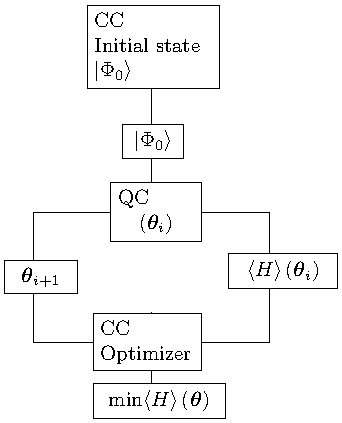
\includegraphics[scale=0.93]{VQE_flow_chart.pdf}
            \end{center}
        \end{column}
    \end{columns}
    

\end{frame}

\end{document} 